% Created 2023-09-22 vi. 18:30
% Intended LaTeX compiler: pdflatex
\documentclass[11pt]{article}
\usepackage[utf8]{inputenc}
\usepackage[T1]{fontenc}
\usepackage{graphicx}
\usepackage{grffile}
\usepackage{longtable}
\usepackage{wrapfig}
\usepackage{rotating}
\usepackage[normalem]{ulem}
\usepackage{amsmath}
\usepackage{textcomp}
\usepackage{amssymb}
\usepackage{capt-of}
\usepackage{hyperref}
\date{\today}
\title{Probing strongly coupled liquids with plasmonics}
\hypersetup{
 pdfauthor={},
 pdftitle={Probing strongly coupled liquids with plasmonics},
 pdfkeywords={},
 pdfsubject={},
 pdfcreator={Emacs 27.2 (Org mode 9.4.4)}, 
 pdflang={English}}
\begin{document}

\maketitle
\tableofcontents


\section{Intro}
\label{sec:orgc32f1f0}

You can find a very simple presentation in these \href{./plasmonics-lecture-notes.pdf}{lecture notes}. These
kind of effects have been known since the 1960s and have been studied
both theoretically and experimentally.


Nowadays, have become even more relevant due to easier access to
experimental techniques. An important advantage they have is due their
sensitivity.


\section{Surface plasmon polaritons (SPP).}
\label{sec:org351a38c}

This is the simplest case of a perfect interface between two different
materials, e.g. air and metal, and solve Maxwell's
equations:


\begin{center}
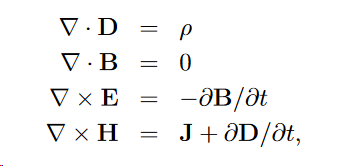
\includegraphics[width=.9\linewidth]{./Surface_plasmon_polaritons_(SPP)/2023-08-22_15-07-26_screenshot.png}
\end{center}

with

\begin{center}
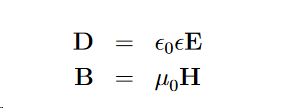
\includegraphics[width=.9\linewidth]{./Surface_plasmon_polaritons_(SPP)/2023-08-22_15-11-15_screenshot.png}
\end{center}

Here one is making implicitly the assumption that \(\epsilon = \epsilon ( \omega)\), otherwise
you would need to account or terms like


\begin{center}
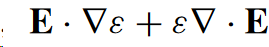
\includegraphics[width=.9\linewidth]{./Surface_plasmon_polaritons_(SPP)/2023-08-22_15-20-39_screenshot.png}
\end{center}

as discussed by \href{./Maier\_PLASMONICS.pdf}{Maier}, after Eq. (2.1)


\begin{center}
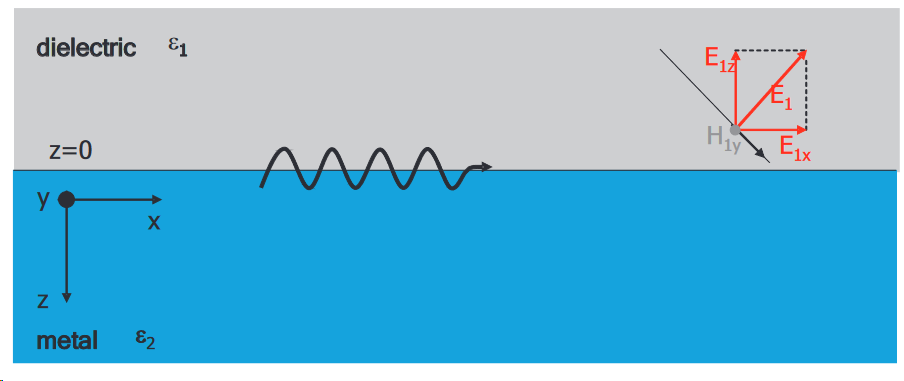
\includegraphics[width=.9\linewidth]{./Surface_plasmon_polaritons_(SPP)/2023-08-21_19-49-35_screenshot.png}
\end{center}


Here the crucial point is that, the dielectric function at a given
frequency has to be negative, leading a mode solution for the TM
(transverse magnetic) polarization that has an evanescent profile
along the axis perpendicular to the plane z, whereas it can still
propagate along the plane.

You start with following plane wave ansatz for each material:


\begin{center}
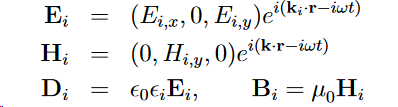
\includegraphics[width=.9\linewidth]{./Surface_plasmon_polaritons_(SPP)/2023-08-22_15-33-50_screenshot.png}
\end{center}


to solve Maxwell's eqs. and the following continuity relation at the
air-metal interface

\begin{center}
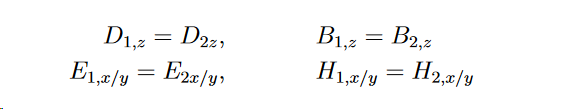
\includegraphics[width=.9\linewidth]{./Surface_plasmon_polaritons_(SPP)/2023-08-22_15-38-37_screenshot.png}
\end{center}



This will have the relation:


\begin{center}
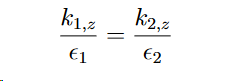
\includegraphics[width=.9\linewidth]{./Surface_plasmon_polaritons_(SPP)/2023-08-22_15-40-20_screenshot.png}
\end{center}

These are indeed imaginary both. The other one left (we took \(k_y=0\)
for simplicity) is the x-component \(k_x\) which is, obviously, the both
materials.


\begin{center}
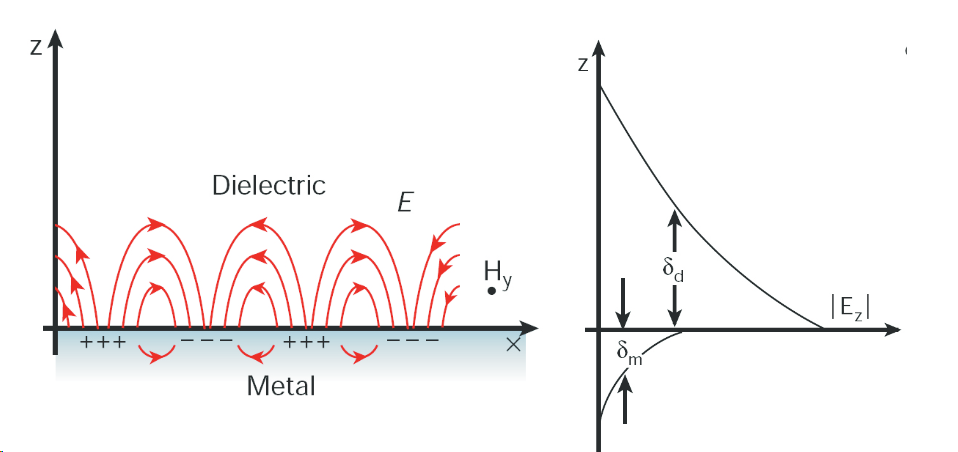
\includegraphics[width=.9\linewidth]{./Surface_plasmon_polaritons_(SPP)/2023-08-22_15-45-12_screenshot.png}
\end{center}



And so the dispersion relation of the mode is given by:



\begin{equation}
k_x^2 = \frac{\omega^2}{c^2 }  \frac{\epsilon_1 \epsilon_2}  {\epsilon_1+ \epsilon_2}
\end{equation}



An argument of why only TM are of interest is given in \href{./Maier\_PLASMONICS.pdf}{Maier}:
\begin{center}
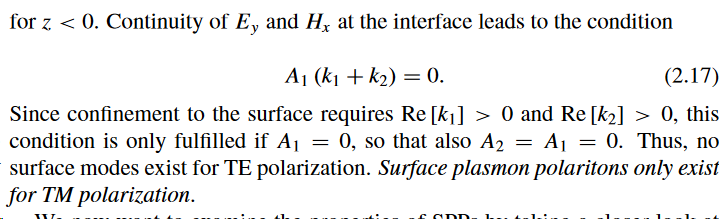
\includegraphics[width=.9\linewidth]{./Surface_plasmon_polaritons_(SPP)/2023-08-21_20-03-10_screenshot.png}
\end{center}




This is applicable for infinite surface case, at least. One might need
to review this also when dealing with a non-local dielectric function.


This is almost always solved using a Drude-like plasmon to the get:


\begin{center}
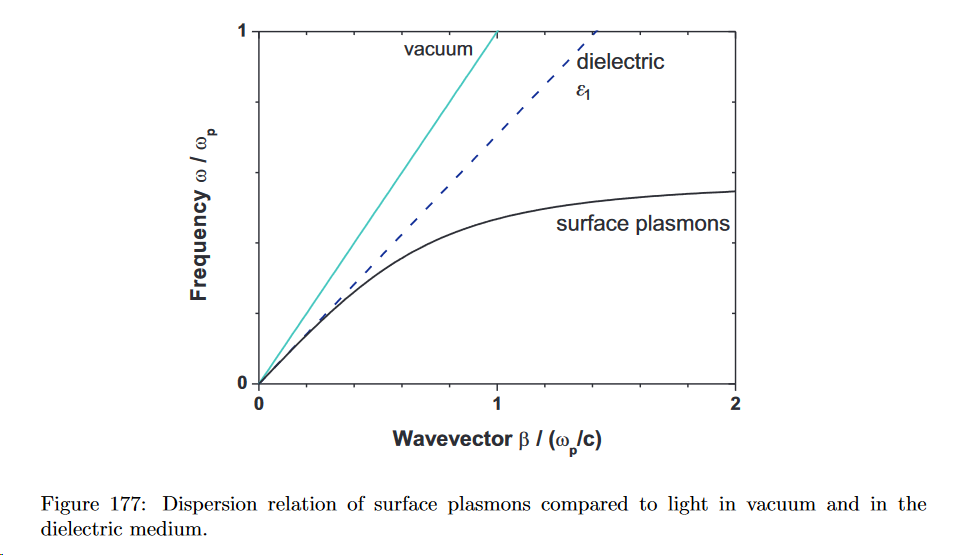
\includegraphics[width=.9\linewidth]{./Surface_plasmon_polaritons_(SPP)/2023-08-22_16-25-56_screenshot.png}
\end{center}



The dielectric line with respect to air or vacuum is important
because SPP don't couple to any modes outside. The only way to excite
them is through a prism of dielectric material whose dielectric
constant is bigger than the air's one, working under total internal
reflection. 




\section{Long-range surface plasmon polaritons}
\label{sec:org0cc5b40}


If, instead semi-infinite metal, you take a thin metal slab,
sandwich between semi-infinite dielectrics:


\begin{center}
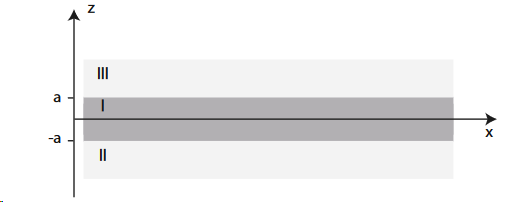
\includegraphics[width=.9\linewidth]{Long-range_surface_plasmon_polaritons/2023-08-25_20-54-57_screenshot.png}
\end{center}


then you get two solutions that are both valid plasmon polaritons, with
the following dispersion (see \href{./Plasmonics-book.pdf}{Plasmonics book}):



\begin{center}
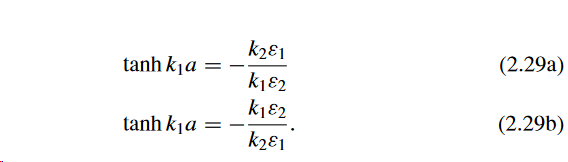
\includegraphics[width=.9\linewidth]{Long-range_surface_plasmon_polaritons/2023-08-25_21-22-38_screenshot.png}
\end{center}






For a plasmon like dielectric function you get:


\begin{center}
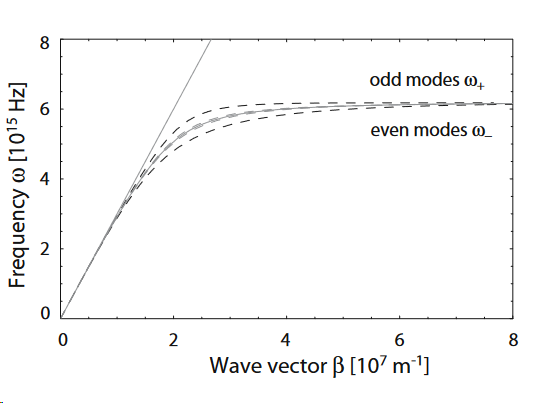
\includegraphics[width=.9\linewidth]{Long-range_surface_plasmon_polaritons/2023-08-25_21-27-24_screenshot.png}
\end{center}

where the upper-mode is known as the long-range spp.



\section{Surface plasmon polaritons (SPP) in 2D.}
\label{sec:org0de3c7a}


Surface plasmon polaritons also show up when considers thin metallic
strips. In a \href{./s41467-020-14826-8.pdf}{recent paper} on quasi-2D-metals, you can see the effect
that has over the shape of the plasmon-polariton dependence on the
wave-vector:


\begin{center}
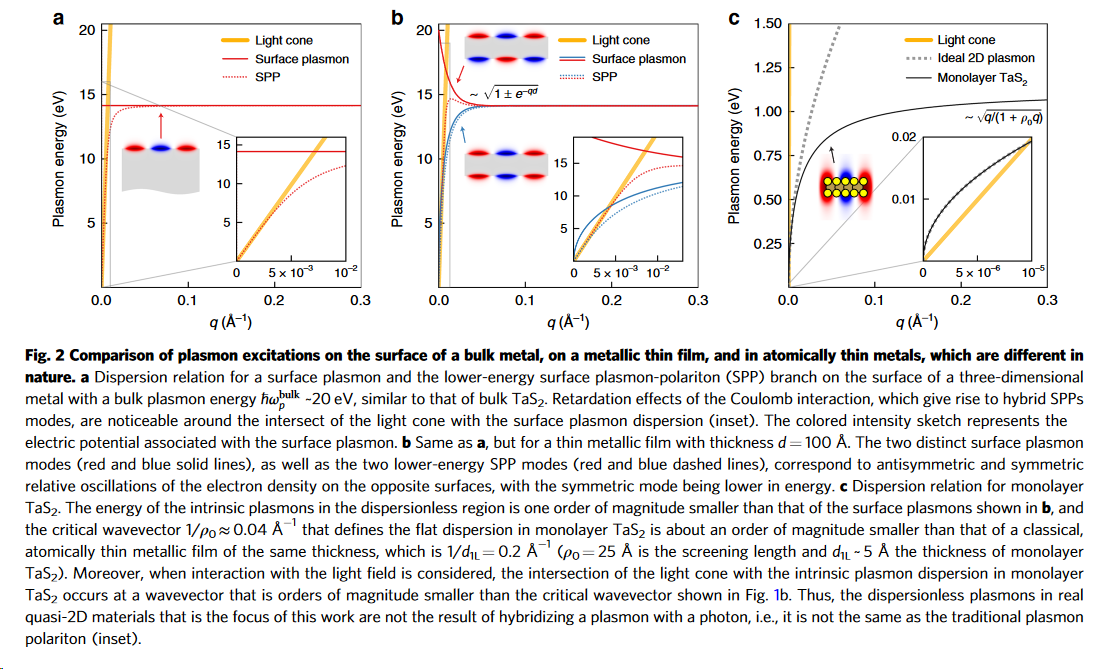
\includegraphics[width=.9\linewidth]{./Surface_plasmon_polaritons_(SPP)_in_2D/2023-08-28_10-34-02_screenshot.png}
\end{center}

Here, panel (a) corresponds to the semi-infinite metal, showing how
the dispersion beds from a flat plasmon to the SPP. Panel (b) same but
a finite-length metallic strip of 100 Angstrom thick, showing both
plasmonic modes. Panel (c) corresponds to a quasi 2D metallic strip,
whose thickness is about 5 Angstrom.

In the latter case, the monolayer shows the standard 2D dispersion

\begin{center}
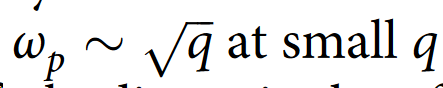
\includegraphics[width=.9\linewidth]{./Surface_plasmon_polaritons_(SPP)_in_2D/2023-08-28_17-43-03_screenshot.png}
\end{center}



Other papers for this 2D case:

\begin{itemize}
\item \href{./1705.07423.pdf}{Observation of surface plasmon polaritons in 2D electron gas}

\item \href{./s41377-022-01012-2.pdf}{Two-dimensional Dirac plasmon-polaritons in graphene, 3D topologicalinsulator and hybrid systems}
\end{itemize}


\begin{itemize}
\item \href{./nanomaterials-13-00975.pdf}{Two-Dimensional Plasmons in Laterally Confined 2D Electron Systems}
\end{itemize}





\section{Papers dealing with spatial dependence for 3D semi-infinite dependence.}
\label{sec:org012def6}


\begin{itemize}
\item \href{https://journals.aps.org/prb/abstract/10.1103/PhysRevB.3.2270}{Surface Plasmon in a Semi-Infinite Free-Electron Gas}

\item \href{./0611257.pdf}{Theory of surface plasmons and surface-plasmon polariton}s
This is more a review than anything but treats the problem self-consistently

\item \href{./0209335.pdf}{Self-consistent solution of the Kohn-Sham equations for systems with inhomogeneous electron gas}

\item \href{./Tokatly\_\_2014\_1015.pdf}{Current-induced spin polarization at the surface of metallic films: a theorem and anab initio calculation}

\item \href{./12-PRB-20-3186-79.pdf}{Conductivity of a semi-infinite electron gas: Effective "optical" surface region}

\item \href{./1511.08708.pdf}{Semi-infinite jellium: Step potential model}
\end{itemize}


\subsection{Sum rules semi-infinite electron gas}
\label{sec:org79a090c}

\begin{itemize}
\item \href{./169.pdf}{The Surface Dielectric Function and Its Sum Rule Semi-Infinite Electrou System}

\item \href{./1511.08708.pdf}{Semi-infinite jellium: Step potential model}
\end{itemize}




\section{Possible problems we could work on}
\label{sec:org6014242}

\begin{itemize}
\item The simplest case would be to deal the 3D case in the
short-wavelength approximation (k=0) for metal or semiconductor, where correlations among
multiple species are important. Remember that we need to have a relatively perfect interface for the
polariton to propagate.
\end{itemize}


\begin{itemize}
\item Next would be a 2D case, where we can work out exactly all
moments for arbitrary wave-number. Especially, if one can probe the case of a bilayer where there is an optic
out-of-phase-mode using plasmon polaritons.

\item Last, work on the full 3D case finding how the moments change with a
semi-infinite metal.
\end{itemize}
\end{document}
